\section{Dynamiczny przydział priorytetów}
\label{ch:alg-priorities-allocation}

Obok algorytmu WHCA* zrealizowano własną metodę dynamicznego przydziału priorytetów oraz skalowania okna czasowego, która pomaga w zwiększeniu skuteczności planowania ruchu robotów. Stanowi to niejako rozwinięcie metody WHCA*.
Układ priorytetów w metodzie WHCA* ma znaczący wpływ na wynik planowania tras. Od priorytetów robotów zależy kolejność wyznaczania tras.
Jest to na tyle istotne, gdyż podczas wyznaczania tras uwzględniane są tylko roboty o priorytetach wyższych (których planowanie odbyło się wcześniej).

Podobnie jak w algorytmie LRA*, również w metodzie WHCA* należy wykrywać kolizje (odpowiednio wcześnie).
Nawet w przypadku, gdy roboty podążają wzdłuż zaplanowanych ścieżek, wciąż mogą zdarzyć się kolizje.
Może to wystąpić w przypadku, gdy robot, który planuje drogę wczesniej (ma wyższy priorytet), nie uwzględnia, że następnemu robotowi może nie udać się wyznaczenie trajektorii (z powodu właśnie zaplanowanej trasy).
Wykrywanie kolizji odbywa się tak samo, jak w przypadku metody LRA* (por. \ref{ch:alg-collision-avoid}).
Należy zaznaczyć, że pod pojęciem wykrywania kolizji rozumiemy wczesne wykrywanie kolizji, która wystąpiłaby w następnym kroku. Nie chcemy doprowadzać do faktycznych kolizji, dlatego interweniujemy odpowiednio wcześniej.

% TODO screen z przypadku kolizjii

Początkowo roboty mają nadane priorytety losowo. Są to kolejne wartości od 1 do liczby wszystkich robotów.
Zaproponowana meotda polega na zwiększaniu priorytetów robotów w przypadku niepowodzenia w znalezieniu trasy.
Opiera się na kilku regułach:
\begin{enumerate}
	\item Przed wykonaniem planowania tras, lista robotów jest sortowana według priorytetów malejąco (wyższa liczba - pierwszeństwo podczas planowania).
	\item Wykonanie planowania tras zgodnie z aktualnym układem kolejnosci robotów.
	\item Jeśli dla któregoś robota nie została znaleziona bezkolizyjna ścieżka, to następuje zwiększenie priorytetu tego robota o wartość 1.
	\begin{enumerate}
		\item Rozmiar okna czasowego zwiększa się do wartości równej maksymalnemu numerowi priorytetu robota.
	\end{enumerate}
	\item Detekcja kolizji dla wszystkich robotów. W przypadku wykrycia, kolejka ruchów obydwu (lub więcej) robotów zostaje zresetowana (opróżniona).
	\item W następnych krokach zostanie podjęta próba ponownego poszukiwania tras dla robotów, u których wystąpiło niepowodzenie planowania lub wykryta kolizja.
\end{enumerate}

Rozszerzanie okna czasowego pozwala na poszukiwanie coraz bardziej skomplikowanych rozwiązań, gdy wciąż nie udaje się znaleźć rozwiązania. Jednocześnie nie przeznaczamy większej mocy obliczeniowej już na początku, gdy prawdopodobnie odbyłoby się planowanie w niepotrzebnie dużej głębi przeszukiwania.

Wykonane testy potwierdziły skuteczność i sens wprowadzeniua metody zarówno dynamicznego przydziału priorytetów jak i rozszerzania okna czasowego dla algorytmu WHCA*.

% TODO przykłady rozwiązywanych problemów
$TODO$
przbieg przypadku z opisem - zwiększanie priorytetów kolejnych krokach

$TODO$ rozróżnienei 3 metod: WHCA*1, WHCA*2, WHCA*3
$TODO$ można skrócić czas planowania, gdy od razu wykonuje się następne planowanie, a nie czeka na kolejny krok
$TODO$ przykład chowania się robotów (przepuszczania się VIPów) - z zaznaczeniem i opisem tras


$TODO$ screeny ciekawych przypadków
\begin{figure}
	\centering
	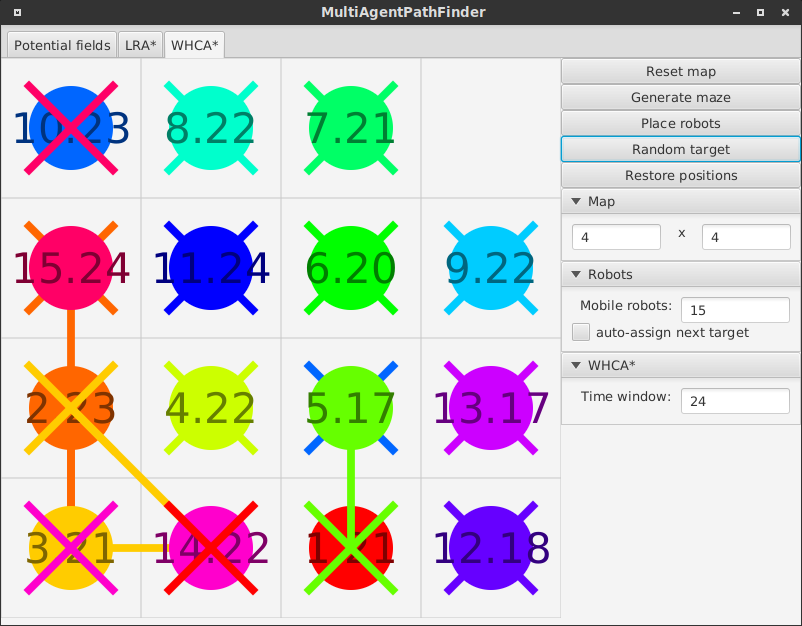
\includegraphics[width=0.8\columnwidth]{img/robopath/puzzle-15}
	\caption{Metoda WHCA*3: puzzle 15}
	\label{fig:test-puzzle-15}
\end{figure}